\begin{frame}{Du masculin au féminin}
  Mets les noms \alert{en gras} au féminin.
  \vspace{0.5cm}
  \begin{columns}
    \column{0.3\textwidth}
      \begin{center}
        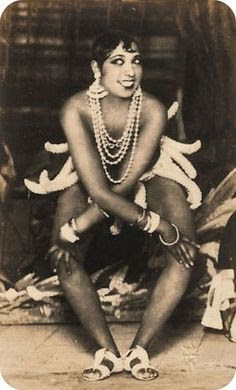
\includegraphics[scale=0.4]{josephine_baker.jpg}
      \end{center}
    \column{0.7\textwidth}
      Joséphine Baker est une \alert{chant\only<-1>{eur}\only<2->{\textcolor{red}{euse}}}, \alert{dans\only<-2>{eur}\only<3->{\textcolor{red}{euse}}}, \alert{ac\only<-3>{teur}\only<4->{\textcolor{red}{trice}}}, \alert{men\only<-4>{eur}\only<5->{\textcolor{red}{euse}}} de revue et \alert{résistant\only<6->{\textcolor{red}{e}}} fran-\\çaise d'origine américaine.
      Elle devient française en 1937 après son mariage avec Jean Lion, un courtier en sucre industriel et un juif -- Baker ne devient ni \alert{cour\only<-6>{tier}\only<7->{\textcolor{red}{tière}}} ni \alert{jui\only<-7>{f}\only<8->{\textcolor{red}{ve}}} elle-même.
      Pendant\\la Seconde Guerre, elle a plusieurs rôles.
      Par exemple, elle participe en tant qu'IPSA (\alert{infirm\only<-8>{ier}\only<9->{\textcolor{red}{ière}}} pilote secouriste de l'air).
      
      % \vspace{1cm}
      % \hyperlink{début}{Au début}...
  \end{columns}
\end{frame}